%!TEX program=xelatex

\documentclass[11pt]{ctexart}  
\usepackage[top=2cm, bottom=2cm, left=2cm, right=2cm]{geometry}  
\usepackage{algorithm}  
\usepackage{algorithmicx}  
\usepackage{algpseudocode}  
\usepackage{amsmath}  
\usepackage{graphicx}
\usepackage{amsmath}
\usepackage{amssymb}


\floatname{algorithm}{算法}
\renewcommand{\algorithmicrequire}{\textbf{输入:}}  
\renewcommand{\algorithmicensure}{\textbf{输出:}} 

\title{密码学实验报告3}
\author{张天辰	17377321}

\makeatletter
\newenvironment{breakablealgorithm}
  {% \begin{breakablealgorithm}
   \begin{center}
     \refstepcounter{algorithm}% New algorithm
     \hrule height.8pt depth0pt \kern2pt% \@fs@pre for \@fs@ruled
     \renewcommand{\caption}[2][\relax]{% Make a new \caption
       {\raggedright\textbf{\ALG@name~\thealgorithm} ##2\par}%
       \ifx\relax##1\relax % #1 is \relax
         \addcontentsline{loa}{algorithm}{\protect\numberline{\thealgorithm}##2}%
       \else % #1 is not \relax
         \addcontentsline{loa}{algorithm}{\protect\numberline{\thealgorithm}##1}%
       \fi
       \kern2pt\hrule\kern2pt
     }
  }{% \end{breakablealgorithm}
     \kern2pt\hrule\relax% \@fs@post for \@fs@ruled
   \end{center}
  }
\makeatother

\begin{document}
\maketitle{}



\section{仿射密码}
\subsection{简介}
仿射密码就是基于$c \equiv a * m + b\quad (\mod 26)$的加密方法,其中要求$\gcd (a, 26) = 1$。

\subsection{算法实现}
\begin{breakablealgorithm}  
    \caption{仿射密码}  
    \begin{algorithmic}[1] %每行显示行号  
        \Require 密钥$a, b$,明文$m$(加密)或密文$c$(解密)  
        \Ensure 密文$c$(加密)或由密钥得到的明文$m'$ 
        \Function {AffineEncrypt}{$message, a, b$} 
            \State $cipher \gets []$
            \For {each $m \in message$}
                \State $cipher.append((a * int(m) + b) \mod 26)$
            \EndFor
            \State \Return $cipher \to string$
        \EndFunction
        \Function {AffineDecrypt}{$cipher, a, b$}
            \State $message \gets []$
            \For {each $c \in cipher$}
                \State $message.append((int(c) - b) * $\Call{reverse}{a}$ \mod 26)$
            \EndFor
            \State \Return $message \to string$
        \EndFunction
    \end{algorithmic}  
\end{breakablealgorithm}
\newpage{}
\subsection{测试样例}
\begin{figure}[htbp]
\centering
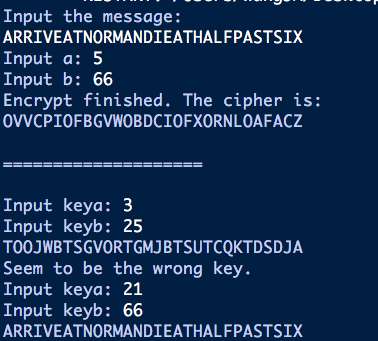
\includegraphics[height=7.56cm,width=6.82cm]{affine.png}
\caption{Affine}
\label{affine}
\end{figure}






\section{Vigenere密码}
\subsection{简介}
此加密方案即将明文和密钥(循环使用)的对应字母相加再模26得到的文字作为密文。
\begin{breakablealgorithm}  
    \caption{Vigenere密码}  
    \begin{algorithmic}[1] %每行显示行号  
        \Require 密钥$key$,明文$message$(加密)或密文$cipher$(解密)  
        \Ensure 密文$cipher$(加密)或明文$message$(解密)
        \Function {VigenereEncrypt}{$message, key$}  
            \State $cipher \gets []$
            \State $lenK \gets len(key)$
            \For {each $i\in [0,len(message))$}
                \State $temp \gets (message[i] + key[i\%lenK]) \mod 26$
                \State $cipher.append(temp)$
            \EndFor
            \State \Return $cipher \to string$
        \EndFunction  
        \Function {VigenereDecrypt}{$cipher, key$}
            \State $message \gets []$
            \State $lenK \gets len(key)$
            \For {each $i \in [0, len(message))$}
                \State $temp \gets cipher[i] - key[i \% lenK]$
                \State $message.append(temp)$
            \EndFor
            \State \Return $message \to str$
        \EndFunction
    \end{algorithmic}  
\end{breakablealgorithm}
\subsection{测试样例}
\begin{figure}[htbp]
\centering
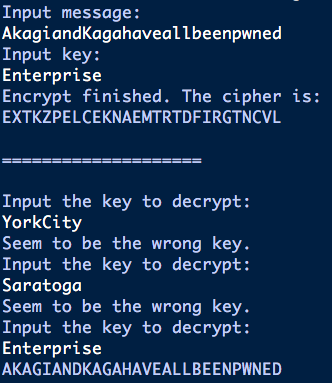
\includegraphics[height=11.49cm,width=9.96cm]{virge.png}
\caption{$Virgenere$}
\label{img_virge}
\end{figure}








\section{Vernam密码}% finish
\subsection{算法简介}
该密码方案将明文和密钥转换为二进制码,然后按位异或(密钥循环)得到密文。解密方法与加密相同。特别地,为了实现中文加密,如果输入语言为中文则每个字符占16位,如果为英文则为8位。
\subsection{算法实现}
\begin{breakablealgorithm}  
    \caption{Vernam密码}  
    \begin{algorithmic}[1] %每行显示行号  
        \Require 密钥$cipher$,明文$message$(加密)或密文$cipher$(解密)  
        \Ensure 明文$message$(解密)或密文$cipher$(加密)
        \Function {VernamEncrypt}{$message, key$}
            \State $cipher \gets []$
            \State $tempm \gets bin(message)$
            \State $tempk \gets bin(key)$
            \State $lenK \gets len(key)$
            \For {each $i \in [0, tempm)$}
                \State $cipher.append(tempm \oplus tempk \to str)$
            \EndFor
            \State \Return $cipher$
        \EndFunction
        \Function {VernamDecrypt}{$cipher, key$}
            \State $message \gets []$
            \State $tempc \gets bin(cipher)$
            \State $tempk \gets bin(key)$
            \State $lenK \gets len(key)$
            \For {each $i \in [0, tempc)$}
                \State $cipher.append(tempc \oplus tempk \to str)$
            \EndFor
            \State \Return $message$
        \EndFunction
    \end{algorithmic}  
\end{breakablealgorithm} 
\subsection{测试样例}
\begin{figure}[htbp]
\centering
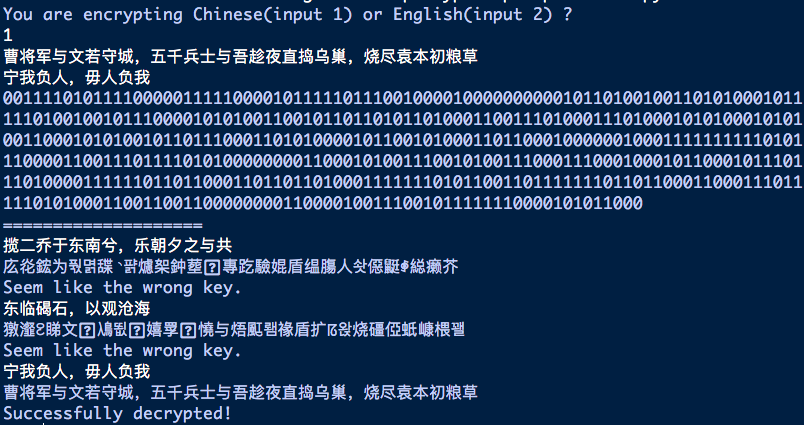
\includegraphics[height=6.37cm,width=12.06cm]{vernam.png}
\caption{$Vernam$}
\label{img_vernam}
\end{figure}

\section{单表代替密码}
\subsection{简介}
利用词频分析可以攻击单表代替密码。通过给不同的字母频率分级并进行枚举猜测,可以实现这种攻击。首先将高频的e,t字母单独处理,在高频的两个密文字母中轮换;再处理a、e、i、o四个中频字母,在四个中频密文字母中轮换;最后按照概率顺序处理其余的所有字母。

输出顺序也与概率相关。因为e概率大于t,a、e、i、o概率依次递减,所以按照全排列生成的顺序就是理论上概率从大到小的顺序。本算法按照这个顺序进行输出。
\subsection{算法实现}
\begin{breakablealgorithm}  
    \caption{Hill密码及其破解}  
    \begin{algorithmic}[1] %每行显示行号  
        \Require 密文$cipher$  
        \Ensure 明文$message$,密钥$key$
        \State $dict\_high \gets e, t$两个高频字母
       	\State $dict\_medium \gets $a, o, i, n四个中频字母
       	\State $dict\_low \gets $其余字母
       	\Function {statistics}{$cipher$}
       		\State $statis \gets {}$
       		\State 将每个字母写入字典的key,出现频率作为value
       		\State $statis$按照value排序
       	\EndFunction
        \Function {crack}{$cipher$}
        	\State $probab \gets $\Call{statistics}{$cipher$}
        	\State $keyd \gets {}$
        	\For {$probab[0, 1]$分别对应e, t}
        		\State 对应写入$keyd$
        		\For {$probab[2, 5]$分别对应a,o,i,n全排列}
        			\State 对应写入$keyd$
        			\State 其余按概率排序分别写入$keyd$
        			\State 对应字典解密,输出
        		\EndFor
        	\EndFor
        \EndFunction     
    \end{algorithmic}  
\end{breakablealgorithm}
\newpage{} 
\subsection{测试样例}
\begin{figure}[htbp]
\centering
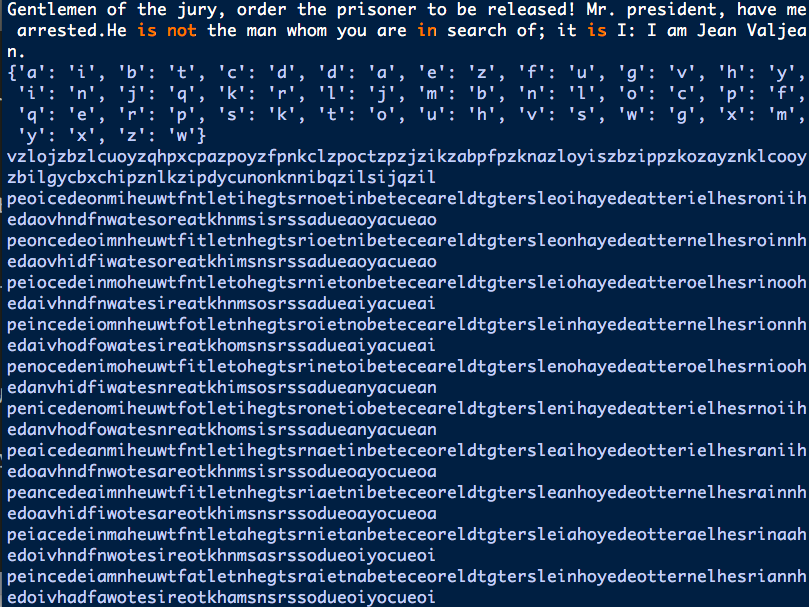
\includegraphics[height=6.07cm,width=8.09cm]{crack.png}
\caption{$SubstitutionCipher$}
\label{img_crack}
\end{figure}


\section{Hill密码}
\subsection{简介}
此加密方案用矩阵作为密钥,对明文消息利用矩阵乘法加密。解密时利用乘矩阵逆元解密。同时,如果获得足够多明密文对,可以对其进行攻击。设明文列向量排成矩阵$M$,其加密结果排成矩阵$C$,密钥为$K$,则有:
$$KM=C\quad K=CM^{-1}$$
可以实现对密钥的攻击。

为了提高程序运行效率,本算法使用python自带函数求解矩阵行列式。如果自己写代码,在矩阵阶数较高(如256)时,其计算量将是惊人的。此外,为了实现支持中文加密,本方案放弃了$\mod 26$的矩阵,而是选择了在$GF_2$上构造矩阵。这样的优点是保证了所有运算能够在域上完成。

矩阵求逆算法采用高斯消元法,复杂度为$O(n^3)$。

\subsection{算法实现}
\begin{breakablealgorithm}  
    \caption{Hill密码及其破解}  
    \begin{algorithmic}[1] %每行显示行号  
        \Require 密钥$cipher$,明文$message$(加密)或密文$cipher$(解密)  
        \Ensure 明文$message$(解密)或密文$cipher$(加密)
        \Function {reverse}{$a, n$}
            \For {each $k \in [0, n)$}
                \State 找到$a[k][k]$及其右下角子式中最大元,并与通过行列变换与$a[k][k]$交换
                \State 交换的行列保存在$rmax[], cmax[]$
                \For {each $j \in [0, n)$}
                    \If {$j \neq k$}
                        $a[k][j] \gets a[k][j] * a[k][k]$
                    \EndIf
                \EndFor
                \For {each $i \in [0, n)$}
                    \If {$i \neq k$}
                        \For {each $j \in [0, n)$}
                            \If {$j \neq k$}
                                $a[i][j] \gets a[i][j] \oplus (a[i][k]*a[k][j])$
                            \EndIf
                        \EndFor
                    \EndIf
                \EndFor
                \For {each $i \in [0, n)$}
                    \If {$i \neq k$}
                        $a[i][k] \gets a[i][k]*a[k][k]$
                    \EndIf
                \EndFor
            \EndFor
            \State 将之前每次循环开始做的行、列变换按照后到先出顺序做其逆变换
            \State \Return $a[][]$
        \EndFunction

        \Function {HillEncrypt}{$key, message, size$}
            \State $intm \gets message \to bit串$
            \State $cipher \gets []$
            \For {$i=0;\;i<len(intm);\;i+=size$}
                $cipher.append(key \dot intm[i:i+size])$
            \EndFor
            \State \Return $cipher \to str$
        \EndFunction

        \Function {HillDecrypt}{$cipher, key, size$}
            \State $intc \gets cipher \to bit串$
            \State $message \gets []$
            \State $key\_1 \to $\Call{reverse}{$key, size$}
            \State $tempk \gets bin(key)$
            \State $lenK \gets len(key)$
            \For {$i=0;\;i<len(intc);\;i+=size$}
                \State $message.append(key\_1 \dot intc[i:i+size])$
            \EndFor
            \State \Return $message \to str$
        \EndFunction

        \Function {HillPwn}{$message, cipher, size$}
            \State $intm \gets message \to bit串$
            \State $intc \gets cipher \to bit串$
            \Repeat
                $message$中取$size^2$bit组成矩阵$m_mat$
                $cipher$中取$size^2$bit组成矩阵$c_mat$
            \Until {$\Call{det}{m\_mat} \neq 0$}
            \State \Return $c\_mat \dot m\_mat$
        \EndFunction
    \end{algorithmic}  
\end{breakablealgorithm} 

\subsection{测试样例}
\begin{figure}[htbp]
\centering
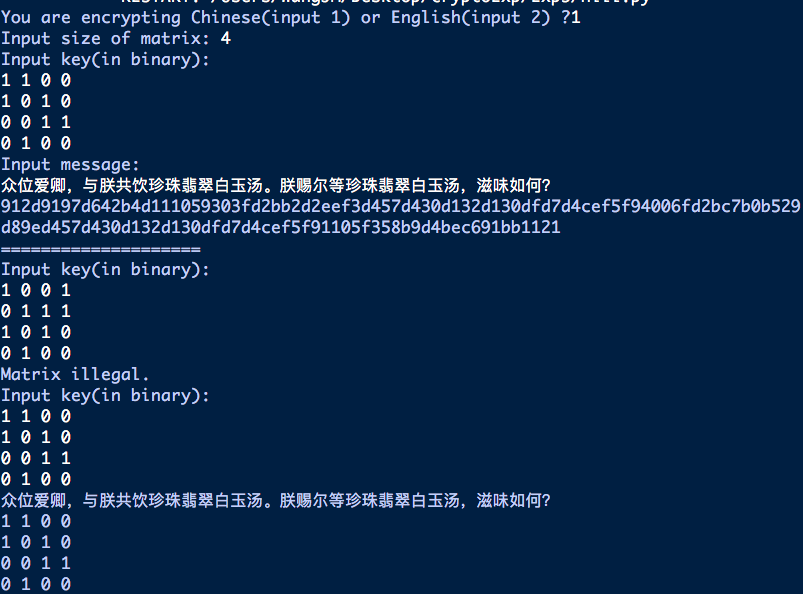
\includegraphics[height=8.91cm,width=12.04cm]{hill.png}
\caption{$Hill$}
\label{img_hill}
\end{figure}

\section{感想}
作业量好大,时间好短。

单表代替密码果然没有那么容易破译,这样破解出来的东西完全没有可读性。如果想要破解这种密码,还是需要语言学家参与进行推断。这样简单的推断还是不够的,需要大量的语言学字典才可以。

希望这门课能变好。
\end{document}